%%%%%%%%%%%%%%%%%%%%%%%%%%%%%%%%%%%%%%%%%
% Jacobs Portrait Poster
% LaTeX Template
% Version 1.0 (31/08/2015)
% (Based on Version 1.0 (29/03/13) of the landscape template
%
% Created by:
% Computational Physics and Biophysics Group, Jacobs University
% https://teamwork.jacobs-university.de:8443/confluence/display/CoPandBiG/LaTeX+Poster
% 
% Further modified by:
% Nathaniel Johnston (nathaniel@njohnston.ca)
% and
% Cameron Smith (@cwsmith on GitHub)
%
% Portrait version by:
% John Hammersley
%
% The landscape version of this template was downloaded from:
% http://www.LaTeXTemplates.com
%
% License:
% CC BY-NC-SA 3.0 (http://creativecommons.org/licenses/by-nc-sa/3.0/)
%
%%%%%%%%%%%%%%%%%%%%%%%%%%%%%%%%%%%%%%%%%

%----------------------------------------------------------------------------------------
%	PACKAGES AND OTHER DOCUMENT CONFIGURATIONS
%----------------------------------------------------------------------------------------

\documentclass[final]{beamer}

\usepackage[size=a1,scale=0.78]{beamerposter} % Use the beamerposter package for laying out the poster

\usetheme{nsfposter} % Use the confposter theme supplied with this template

\setbeamercolor{block title}{fg=ngreen,bg=white} % Colors of the block titles
\setbeamercolor{block body}{fg=black,bg=white} % Colors of the body of blocks
\setbeamercolor{block alerted title}{fg=white,bg=dblue!70} % Colors of the highlighted block titles
\setbeamercolor{block alerted body}{fg=black,bg=dblue!10} % Colors of the body of highlighted blocks
% Many more colors are available for use in beamerthemeconfposter.sty

%-----------------------------------------------------------
% Define the column widths and overall poster size
% To set effective sepwid, onecolwid and twocolwid values, first choose how many columns you want and how much separation you want between columns
% In this template, the separation width chosen is 0.024 of the paper width and a 4-column layout
% onecolwid should therefore be (1-(# of columns+1)*sepwid)/# of columns e.g. (1-(4+1)*0.024)/4 = 0.22

\newlength{\sepwid}
\newlength{\onecolwid}
\setlength{\paperwidth}{23.4in} % A1
\setlength{\paperheight}{33.1in} % A1
\setlength{\sepwid}{0.024\paperwidth} % Separation width (white space) between columns
\setlength{\onecolwid}{0.30\paperwidth} % Width of one column
\setlength{\topmargin}{-0.5in} % Reduce the top margin size
%-----------------------------------------------------------

\usepackage{graphicx}  % Required for including images

%algorithms and pseudo code
\usepackage{algorithm}
\usepackage[noend]{algpseudocode}

%----------------------------------------------------------------------------------------
%	TITLE SECTION 
%----------------------------------------------------------------------------------------

\title{Fast Dynamic Load Balancing Tools for Extreme Scale Systems} % Poster title

\author{PI: Mark S. Shephard, Co-PI: Cameron W. Smith} % Author(s)

\institute{Scientific Computation Research Center (SCOREC) at Rensselaer Polytechnic Institute, Troy, NY, USA} % Institution(s)

%----------------------------------------------------------------------------------------

\begin{document}

\addtobeamertemplate{block end}{}{\vspace*{2ex}} % White space under blocks
\addtobeamertemplate{block alerted end}{}{\vspace*{2ex}} % White space under highlighted (alert) blocks

\setlength{\belowcaptionskip}{2ex} % White space under figures
\setlength\belowdisplayshortskip{2ex} % White space under equations

\begin{frame}[t] % The whole poster is enclosed in one beamer frame

\begin{columns}[t] % three columns

\begin{column}{\sepwid}\end{column} % Empty spacer column

\begin{column}{\onecolwid} % The first column

%----------------------------------------------------------------------------------------
%	OBJECTIVES
%----------------------------------------------------------------------------------------

\begin{alertblock}{Motivation and Focus}
  GPUs provide >90\% of the compute power on leadership systems.\\
  Simulations with regions of physical interest that change can have\\
  \begin{itemize}
    \item complex relational structures,
    \item irregular forms of computational \& communication costs, and
    \item evolving imbalance of work characterized by multiple criteria.
  \end{itemize}
  Provide fast dynamic load balancing on GPUs where simulation data exists. \\
  \vskip1cm
  \includegraphics[width=.45\textwidth]{../salishan2019/figures/xgcCase.png}
  \includegraphics[width=.45\textwidth]{../salishan2019/figures/laghos_sedov.png}\\
  \small{XGC fusion plasma physics (left) and MFEM Laghos Sedov blast
  (right).}
\end{alertblock}

%------------------------------------------------

%\begin{block}{Accelerated Systems}
%  \begin{itemize}
%    \item Host processor - dispatches accelerator work, facilitates
%      communications, OS interactions
%    \item Accelerator - provides most of the computing power \\
%      e.g.) ORNL Summit GPUs have 95\% of memory bandwidth and 98\% of FLOPs
%  \end{itemize}
%\end{block}
%\begin{figure}
%  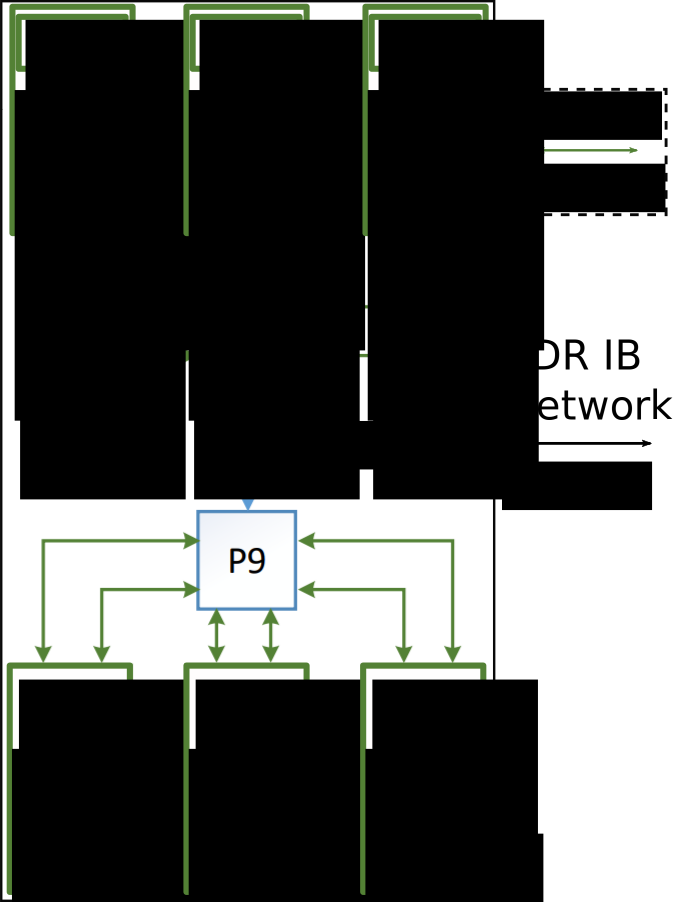
\includegraphics[width=.5\textwidth]{../salishan2019/figures/summit-node.png}\\
%  \small{ORNL Summit Compute Node: IBM AC922}\\
%  \tiny{J.Choquette. Hot Chips 2017. "Volta: Programmability and Performance"}
%\end{figure}
%
%\begin{block}{Common Methods for Partitioning and Load Balancing}
%\end{block}
%\begin{figure}
%  \centering
%  \includegraphics[width=.3\textwidth]{../salishan2019/figures/mitchellMesh.png}
%  \includegraphics[width=.3\textwidth]{../salishan2019/figures/mitchellHSFC.png}
%  \includegraphics[width=.3\textwidth]{../salishan2019/figures/mitchellRCB.png} \\
%  \includegraphics[width=.3\textwidth]{../salishan2019/figures/mitchellRIB.png}
%  \includegraphics[width=.3\textwidth]{../salishan2019/figures/mitchellParmetis.png} \\
%  \small{Top to bottom, left to right: mesh, space filling curve,
%  coordinate bisection, inertial bisection, multi-level k-way.} \\
%  \tiny{``A refinement-tree based partitioning method for dynamic load
%  balancing with adaptively refined grids'', William F. Mitchell}
%\end{figure}


%----------------------------------------------------------------------------------------

  
\begin{block}{What is EnGPar?}
   \begin{itemize}
     \item Provides a diffusive load balancing algorithm for partition improvement and supports multi-criteria partitioning.
     \item Complements existing multi-level and geometric methods.
     \item Utilizes a weighted multi(hyper)graph structure to represent
       data dependencies.
     \item Implemented to support efficient data parallel operations on accelerators
   \end{itemize}
   \includegraphics[width=.24\textwidth]{../salishan2019/figures/engparDiffusion/0.jpg}
   \includegraphics[width=.24\textwidth]{../salishan2019/figures/engparDiffusion/1.jpg}
   \includegraphics[width=.24\textwidth]{../salishan2019/figures/engparDiffusion/2.jpg}
   \includegraphics[width=.24\textwidth]{../salishan2019/figures/engparDiffusion/3.jpg}
   \includegraphics[width=.24\textwidth]{../salishan2019/figures/engparDiffusion/4.jpg}
   \includegraphics[width=.24\textwidth]{../salishan2019/figures/engparDiffusion/5.jpg} \\
   Multiple diffusive iterations (left to right) biased
   to migrate entities in order of descending distance (red to blue) from the
   topological center of the part (blue).
\end{block}

\begin{block}{Unstructured Mesh Partition Improvement}
  \medskip
  Problem setup
  \begin{itemize}
    \item Billion element mesh of vertical tail structure.
    \item Run on the Mira BG/Q with one process per hardware thread.
    \item Target imbalance of 1.05.
    \item The imbalance of a given type (vtx, edge,
      face, or region) is defined as the max part
      weight divided by the avg part weight.
  \end{itemize}
  Initial partitions are built using:
  \begin{itemize}
  \item Global ParMETIS part k-way to 8Ki($8*2^{10}$) parts.
  \item Local ParMETIS part k-way from 8Ki to 128Ki, 256Ki, and 512Ki parts.
  \end{itemize}
\end{block}

\end{column} % End of the first column

\begin{column}{\sepwid}\end{column} % Empty spacer column

\begin{column}{\onecolwid} % The second column


\begin{block}{Element Partition: Mesh Vertex Imbalance Reduction}
  The partitions before using EnGPar:\\
  \begin{table}[!h]
    \small
    \centering
    \begin{tabular}{||c|c|c|c||}
      \hline
      Number of Parts &128Ki&256Ki&512Ki \\
      \hline
      Elements per part & 9,836 & 4,918&2,459  \\
      \hline
      Vertex imbalance & 1.13 & 1.18 & 1.53 \\
      \hline
      Element imbalance & 1.02& 1.02& 1.02\\
      \hline
    \end{tabular}
  \end{table}
  {\centering
    \includegraphics[width=.6\textwidth]{../accelerated_cse19/figures/elmPtn_vtxImb.png}
    \includegraphics[width=.6\textwidth]{../accelerated_cse19/figures/elmPtn_elmImb.png} \\
    Mesh vertex imbalances are reduced from 13\% to 5\% for 128Ki, 18\% to 5\% for
    256Ki, and 53\% to 6\% for 512Ki.  Edge cut is increased by 1\%.
  }
\end{block}


\begin{block}{Diffusive Partitioning}
  \begin{algorithm}[H]
    \caption{Diffusive Load Balancing Framework}
    \label{alg:engpar}
    \small
    \begin{algorithmic}[1]
      \Procedure{Balance}{$ngraph$,$entity\_types$}
      \ForAll{$t \in entity\_types$}
      \While{imbalance of $t >$ tolerance}
      \Call{RunStep}{$ngraph$,$t$}
      \If{Balancing Stagnates}
      \State break
      \EndIf
      \EndWhile
      \EndFor
      \EndProcedure

      \Procedure{RunStep}{$ngraph$,$t$}
      \State $sides = makeSides(ngraph)$
      \State $weights = makeWeights(ngraph,sides,t)$
      \State $targets = makeTargets(ngraph,sides,weights)$
      \State $queue = makeQueue(ngraph)$
      \State $plan = select(ngraph,targets,queue)$
      \State $ngraph.migrate(plan)$
      \EndProcedure
    \end{algorithmic}
  \end{algorithm}
\end{block}

\begin{block}{Queue}
  One inward BFS and one outward BFS to compute graph distance; the traversal
  order.
  \begin{figure}
    \centering
    \includegraphics[width=.4\textwidth]{../accelerated_cse19/figures/2dTreeDepth.png}
    \includegraphics[width=.41\textwidth]{../accelerated_cse19/figures/2dDistance.png}
  \end{figure}
      (left) The distance from each vertex to the boundary and (right) the
    distance from the core vertex (marked with a zero near the
    bottom left corner).
\end{block}

\begin{figure}
  \centering
  \includegraphics[width=.9\textwidth]{../accelerated_cse19/figures/sellcsigma.png}\\
  Sell-C-Sigma structure (Besta and Merending, et al.)
\end{figure}


\end{column} % End of the second column
\begin{column}{\sepwid}\end{column} % Empty spacer column
\begin{column}{\onecolwid} % The third column

\begin{block}{Accelerating BFS}
  Hypergraphs created from unstructured tet mesh of automotive part \\
  Timing comparison on NVIDIA 1080ti - includes data transfers, but not JIT; 
  average of three runs shown \\
  \texttt{scg\_int\_unroll} is 4.78 times faster than csr on 28M graph and up to 
      11 times faster than serial push on Intel Xeon (not shown) \\
  Memory coalescing is critical; csr vs. scg \\
  {
    \centering
    \includegraphics[width=.97\textwidth]{../accelerated_cse19/results/openclBfs.png} \\
    { \small
    \texttt{push}: C++ serial push,
    \texttt{pull}: C++ serial `pull',
    \texttt{csr}: OpenCL `pull' on CSR, 
    \texttt{scg}: OpenCL `pull' on Sell-C-Sigma,
    \texttt{*\_int}: 4B int,
    \texttt{*\_unroll}: unroll the vtx-to-hyperedge loop
    }
  }
\end{block}

\begin{block}{Selection using Kokkos}
  Operate on non-overlapping cavities to avoid race; color the boundary \\
  A cavity is selected for migration if it satisfies color, target, and size
  criteria \\
  { \centering
    \includegraphics[width=\textwidth]{../accelerated_cse19/figures/kkColoringAndDual.png}\\
    Speedup of parallel vs. serial coloring and dual computation on NVIDIA 1080ti
  }
  Making good decisions
  { \centering
    \includegraphics[width=\textwidth]{../accelerated_cse19/figures/selectionEx.png}\\
    Initial, GPU Selection, CPU Selection
  }
  Bias selection towards cavities with highest topological distance.
\end{block}

\begin{block}{Closing Remarks and Future Work}
  \begin{itemize}
    \item Using Kokkos for improved portability and ease of use over OpenCL
    \item Porting of BFS to Kokkos is underway
    \item Focused on balancing particles in XGCm accelerated unstructured mesh PIC
  \end{itemize}
\end{block}

\begin{block}{More Info}
  EnGPar - \url{github.com/SCOREC/EngPar} \\
  Mark S. Shephard - \url{shephard@rpi.edu} \\
  Cameron W. Smith - \url{smithc11@rpi.edu} \\
\end{block}



\end{column} % End of the third column

\begin{column}{\sepwid}\end{column} % Empty spacer column

\end{columns} % End of all the columns in the poster

\end{frame} % End of the enclosing frame

\end{document}
